\chapter{Marco teórico} \label{cap:dos}

Todo proyecto de software se desencadena por alguna necesidad de negocios: la de corregir un defecto en una aplicación existente, la de adaptar un “sistema heredado” a un ambiente de negocios cambiante, la de ampliar las funciones y características de una aplicación ya existente o la necesidad de crear un producto, servicio o sistema nuevo.
Al comenzar un proyecto de software, es frecuente que las necesidades del negocio se expresen de manera informal como parte de una simple conversación.  El esfuerzo de ingeniería tendrá éxito sólo si también lo tiene el software. El mercado aceptará el producto sólo si el software incrustado en éste satisface las necesidades del cliente.

\section{Ingeniería de software}

Una de las primeras definiciones de ingeniería de software fue dada por Fritz Bauer en el año de 1969, quien define que la ingeniería de software es..\\

	\textit {“el establecimiento y uso de principios robustos, orientados a obtener software económico que sea fiable y que funcione de manera eficiente sobre máquinas reales” }. \\
	
  Aunque esta definición omite algunos términos referentes a tiempos de entrega, procesos eficaces, y calidad de software, nos da un panorama de sus principios fundamentales y es también la base de la definición que la IEEE ha desarrollado de una manera más completa: \\

 \textit {"La ingeniería de software es: La aplicación de un enfoque sistemático, disciplinado y cuantificable al desarrollo, operación y mantenimiento de software; es decir, la aplicación de la ingeniería al software.”}  \hyperlink{b07}{[7]}\\

La ingeniería de software está formada por un proceso, un conjunto de métodos (prácticas) y un arreglo de herramientas que permite a los profesionales elaborar software de cómputo de alta calidad. 

Un aspecto muy importante de Ingeniería de Software es que proporciona parámetros formales para lo que se conoce como Gestión (o Administración) de Proyectos de Software. Esto se refiere a que Ingeniería de Software proporciona diversas métricas y metodologías que pueden usarse como especificaciones para todo lo referente a la administración del personal involucrado en proyectos de software, ciclos de vida de un proyecto de software, costos de un proyecto, y en si todo el aspecto administrativo que
implica el desarrollar software.\\

La ingeniería en general es el análisis, diseño, construcción, verificación y gestión de entidades técnicas. En general, todo proceso de ingeniería debe comenzar por contestar las siguientes preguntas: ¿Cuál es el problema a
resolver?, ¿Cuáles son las características de la entidad que se utiliza para resolver el problema?, ¿Cómo se realizará la entidad (y la solución)?, ¿Cómo se construirá la entidad?, ¿Cómo va a probarse la entidad?, y ¿Cómo se apoyará la entidad cuando los
usuarios finales soliciten correcciones y adaptaciones a la entidad?.  \hyperlink{b07}{[7]}  \\

\begin{figure}[H]
	\begin{center}
		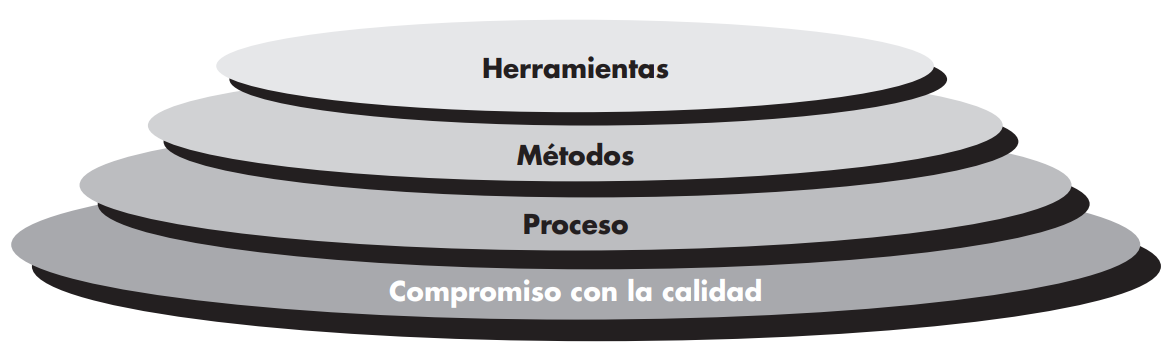
\includegraphics[width=.95\textwidth]{images/CapasIS}
		\caption{Capas de la ingeniería de software}
		\label{fig:capas_is}
	\end{center}
\end{figure}

La ingeniería de software es una tecnología con varias capas, como se muestra en la figura 3.1, existen 4 capas: herramientas, métodos, procesos y compromiso con la calidad. Cada una de ellas es importante, sin embargo, la capa de proceso es fundamental para el desarrollo de software, ya que es donde se define la estructura básica del producto hasta la culminación del mismo.

El proceso de software forma la base para el control de la administración de proyectos de software, y establece el contexto en el que se aplican métodos técnicos, se generan productos del trabajo (modelos, documentos, datos, reportes, formatos, etc.), se establecen puntos de referencia, se asegura la calidad y se administra el cambio de manera apropiada.

\section{Proceso de desarrollo de software}

Se define proceso del software como una estructura para las actividades, acciones y tareas que se requieren a fin de construir software de alta calidad. La ingeniería de software es llevada a cabo por personas creativas y preparadas que deben adaptar un proceso maduro de software a fin de que resulte apropiado para los productos que construyen y para las demandas de su mercado.
Cuando se trabaja en la construcción de un producto o sistema, es importante ejecutar una serie de pasos predecibles, una estructura general para la ingeniería de software se define en cinco actividades elementales:

\begin{enumerate}
	\item Comunicación
	\item Planeación
	\item Modelado
	\item Construcción
	\item Despliegue
\end{enumerate}

Existen diferentes metodologías de desarrollo con modificaciones y adecuaciones al esquema general de construcción antes mencionado, algunas de ellas son las metodologías tradicionales y ágiles. Este proceso puede tener diferentes variaciones, sin embargo, sea cual sea la metodología aplicada, las etapas de Modelado (Análisis y Diseño) y Costrucción (Codificación y Pruebas) son las más críticas e importantes para un producto final exitoso.

Durante el desarrollo, se realizan tareas específicas para cada etapa, por ejemplo, para la etapa de modelado se elabora el documento de análisis (donde se describe el funcionamiento del sistema), así como el diseño (en donde se genrean los diagramas que describen el funcionamiento establecido en el análisis); en la fase de construcción se genera el código del software y en la etapa de pruebas se valida y verifica que el software cumpla con lo asentado en las fases precedentes.

\subsection{Análisis}

El proceso de análisis dentro del desarrollo de software consiste en obtener los requerimientos del sistema para crear una solución, identificar los problemas a resolver o necesidad a ser atendida, evaluar las restricciones que presenta, así como los insumos se requieren para su debida construcción.
Al ser la primera etapa dentro del proceso de desarrollo es las más crítica y sensible, ya que cualquier error de gran impacto que surja dentro de esta perjudicará las etapas consecuentes ocasionando retrasos en el proceso.

\bigskip

En esta etapa se construye el documento de análisis, en donde se describen todos los requerimientos que el cliente ha solicitado mediante diferentes componentes
Con base en los requisitos, el analista sigue el proceso de análisis identificando en alto nivel que funcionalidades deberá poseer el sistema para cumplir los requerimientos. Una solución común para mapear cada funcionalidad es a través de CASOS DE USO.

Este documento emplea un lenguaje técnico especializado ya que busca ser comprendido por los diseñadores y programadores para su correcta construcción.

\subsubsection{Documento de análisis}

Parte 1. Modelo de negocio:
Glosario de términos
Modelo de información utilizado para representar la información que será almacenada en el sistema.
Reglas de negocio mediante las cuales se normará el funcionamiento del sistema.
Parte 2. Modelo dinámico, el cual describe funcionalidad a partir de los siguientes capítulos:
Arquitectura lógica.
Máquinas de estados que modelarán el comportamiento de las entidades que así lo necesiten.
Funciones y roles que tendrán los actores que interactuarán con el sistema.
Casos de uso que describen funcionalidad.
Parte 3. Interacción con el usuario, que muestra las interfaces y mensajes a partir de los siguientes
capítulos:
Interfaces del sistema.
Catálogo de mensajes

\subsubsection{Caso de Uso}

Un caso de uso es una actividad que puede realizar un usuario dentro del software. Estas actividades sirven para describir el comportamiento del producto en distintas condiciones en las que el sistema responde a alguna de las peticiones realizadas por el usuario, es decir, describe el funcionamiento de los componentes acorde a las acciones que los usuarios realizan dentro del software.

En un libro que analiza cómo escribir casos de uso eficaces, Alistair Cockburn [Coc01b] afirma que “un caso de uso capta un contrato […] [que] describe el comportamiento del sistema en distintas condiciones en las que el sistema responde a una petición de alguno de sus participantes[…]”.

En esencia, un caso de uso narra una historia estilizada sobre cómo interactúa un usuario final (que tiene cierto número de roles posibles) con el sistema en circunstancias específicas. La historia puede ser un texto narrativo, un lineamiento de tareas o interacciones, una descripción basada en un formato o una representación diagramática. Sin importar su forma, un caso de uso ilustra el software o sistema desde el punto de vista del usuario final.

Un caso de uso está compuesto por distintos elementos, los cuales se describen a continuación:
\begin{itemize}
\item \textbf{Actor}: Es la idealización de un rol que puede jugar una persona, otro sistema, proceso, un dispositivo o de alguna cosa que interactúa con el sistema. Los actores son objetos que residen fuera del sistema, en tanto que los casos de uso están compuestos por objetos y acciones que residen dentro del sistema. Todo actor tiene uno o más objetivos cuando utiliza el sistema.  \hyperlink{b09}{[9]}. 

\item \textbf{Entidad} : Representación de un objeto exclusivo único en el mundo real que se está controlando. Algunos ejemplos de entidad son una sola persona, un solo producto o una sola organización. 

\item \textbf{Atributo} : Es una especificación que define una propiedad de un objeto, elemento o archivo. También puede referirse o establecer el valor específico para una instancia determinada de los mismos.

\item \textbf{Entrada}: Es la información producida por el usuario para ser guardada o procesada en el sistema. El usuario comunica y determina qué clases de entrada aceptará el sistema (por ejemplo, secuencias de control o de texto escritas a máquina a través del teclado y el ratón).

\item \textbf{Salida}: Es la información producida por el sistema y percibida por el usuario. Las clases de salida los productos de programa, y las clases de entrada la que el programa acepta, definen la interfaz de usuario del programa.

\item \textbf{Acción}: Evento originado por el usuario mediante botones.

\item \textbf{Pantalla}: Es la interfaz de usuario, utiliza imágenes, iconos y menús para mostrar las acciones disponibles entre las que el usuario puede escoger en un sistema. Su función es proporcionar un entorno visual amigable y sencillo de usar que facilite la comunicación del usuario con el software.

\item \textbf{Regla de Negocio}: Es aquella que rige los procesos de un negocio para garantizar el correcto funcionamiento del software. Las reglas de negocio establecen los procedimientos que se deben realizar y las condiciones sobre las que dichas actividades se van a ejecutar.

\item \textbf{Mensaje}: Constituyen la mínima unidad de comunicación entre el usuario y el sistema. Se trata de un proceso de comunicación completa porque el sistema lanza un mensaje hacia el usuario que no se resuelve hasta que el usuario lo recibe o lo responde, completando así el proceso de comunicación con la realimentación correspondiente.

\item \textbf{Trayectoria}: Es un conjunto de pasos que describen la interaccion entre el usuario y el sistema.

\item \textbf{Paso}: Es una instruccion que realiza el usuario o el sistema.

\item \textbf{Precondición}: Está formada por el conjunto de condiciones que se tienen que cumplir para que se pueda iniciar un caso de uso. En muchos casos supone la ejecución de casos de uso previos.

\item \textbf{Postcondición}: Refleja el estado en que se queda el sistema una vez ejecutado el caso de uso.

\item \textbf{Puntos de extensión}: Es la incorporación implícita del comportamiento de otro caso de uso, el cuál no es parte del flujo principal. Modela la parte opcional del sistema, un subflujo que sólo se ejecuta bajo ciertas condiciones o varios flujos que se pueden insertar en un punto determinado. 
\end{itemize}